\begin{figure}[htb]
  \centering
%segundo bloco de figuras
  \begin{tabular}{c c c c c }
    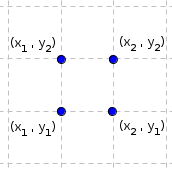
\includegraphics[width=3.5cm]{./img/dispositionFrameInGrid.png}    
    %& &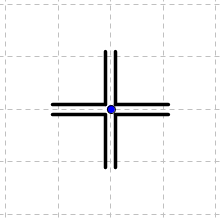
\includegraphics[width=4cm]{./img/truePieGrid.png} 
    & &
 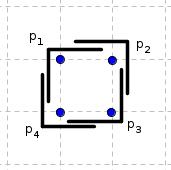
\includegraphics[width=3.5cm]{./img/frameInGrid.png} \\%[\abovecaptionskip]
    {\footnotesize (a) Points of the coordinates of bends of a frame}  
    %& &  {\footnotesize (b) True pie} 
    & & {\footnotesize (c) Paths of a frame} %\label{fig:frame}
  \end{tabular}
  \caption{$B_{1}$-EPG representation of the induced cycle of size 4 as frame}\label{fig:frameInGrid}
\end{figure} 